\subsection*{A Generic BVP}

\begin{frame}[t]
  \begin{columns}[t]
    \column{.5\textwidth}
     \begin{itemize}
      \item Common BVP components:
      \vspace{-.1in}
        \begin{eqnarray}
        \label{eqn:general_pde}
        \nonumber
        \bv{M} \frac{\partial \bv{u}}{\partial t} & = & \bv{F}( \bv{u} ) \;\, \in \Omega \subset \Reals^n
        \\
        \nonumber
        \bv{G}( \bv{u} ) & = & 0 \;\;\;\;\;\;\;\; \in \Omega
        \\
        \nonumber
        \bv{u} & = & \bv{u}_D \;\;\;\;\; \in \partial \Omega_D
        \\
        \nonumber
        \bv{N}(\bv{u}) & = & 0 \;\;\;\;\;\;\;\; \in \partial \Omega_N
        \\
        \nonumber
        \bv{u}(\bv{x}, 0) & = & u_0(\bv{x}) 
      \end{eqnarray}
      \item Less common components:
        \begin{itemize}
        \item Moving domain $\Omega(t)$, $\Omega(\bv{u},t)$
        \item Multi-dimensional manifolds
        \item Self-overlapping, contact
        \item Acceleration ${\partial^2 u}/{\partial t^2}$
        \item Integro-differential equations
        \end{itemize}
      \end{itemize}
    \column{.5\textwidth}
      \begin{center}
        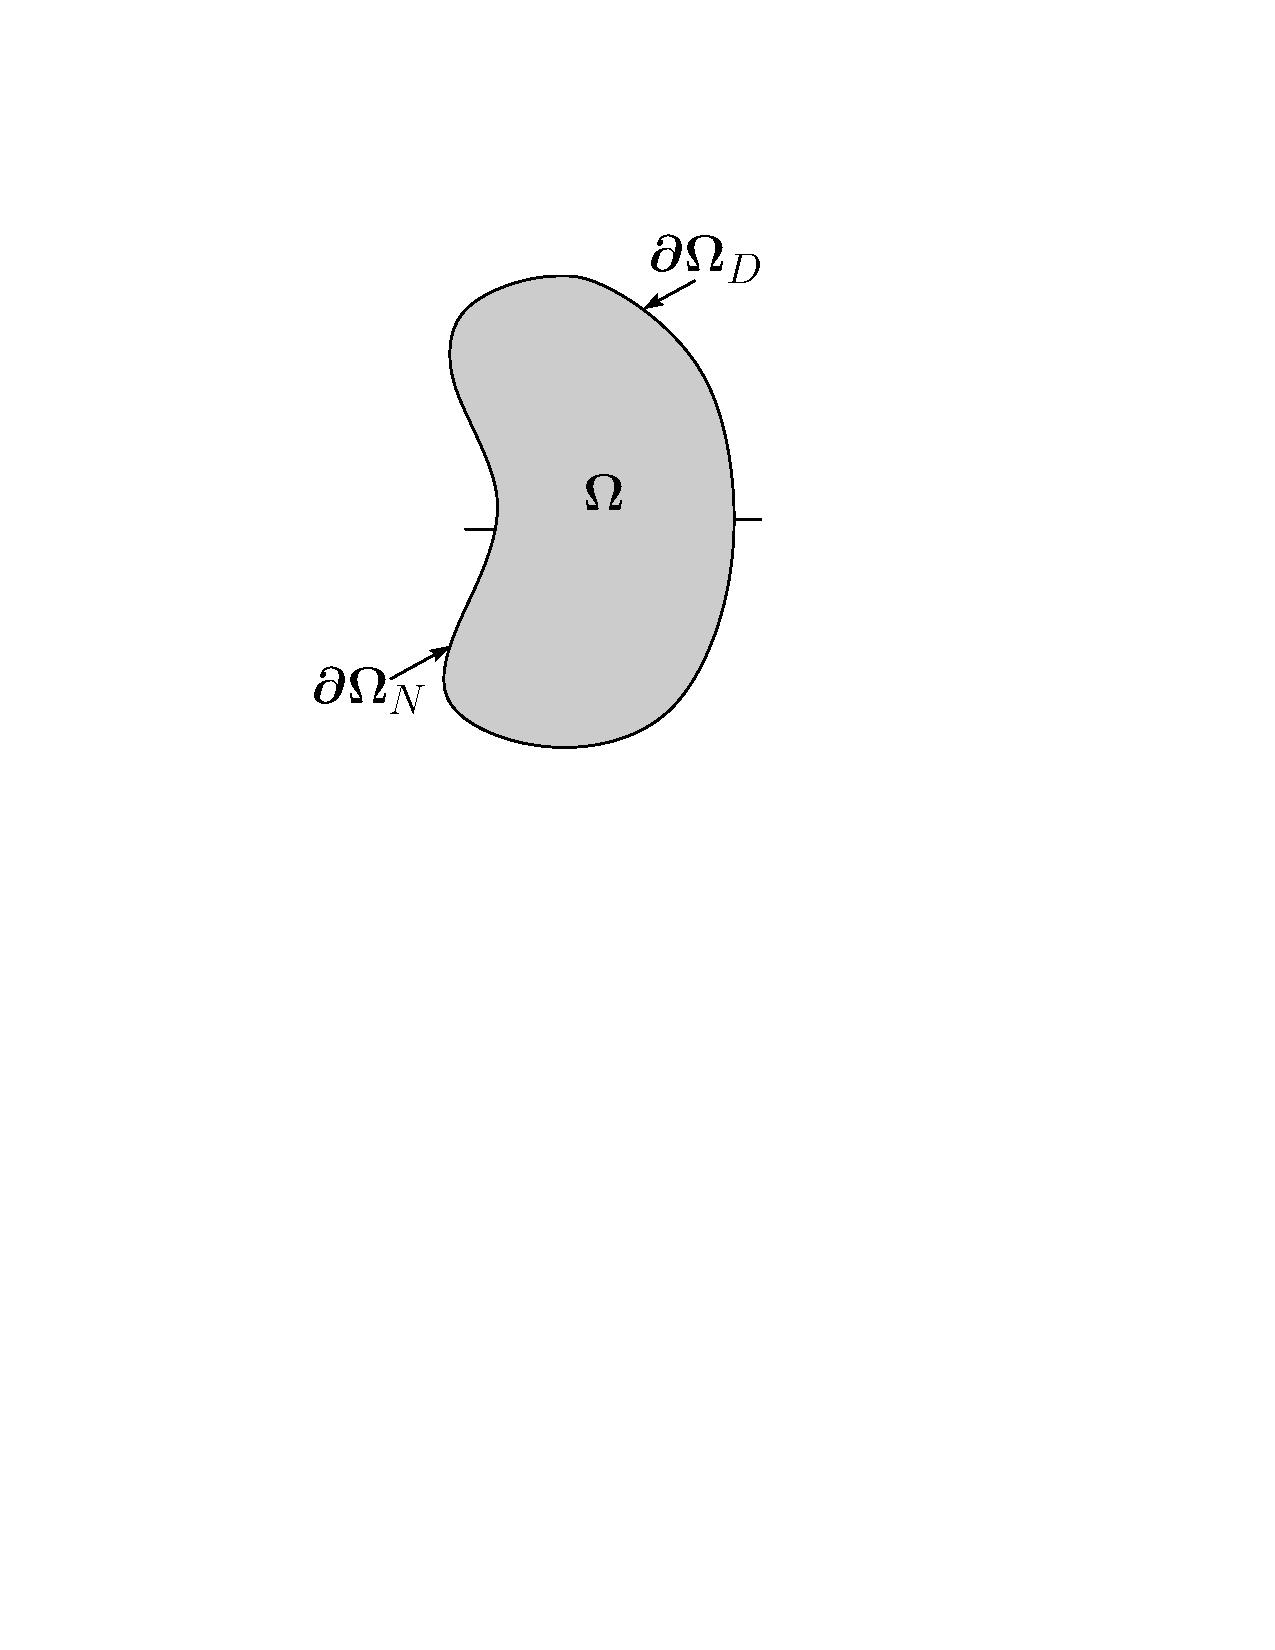
\includegraphics[viewport=140 420 400 685,clip=true,width=.45\textwidth]{domain2_input}
        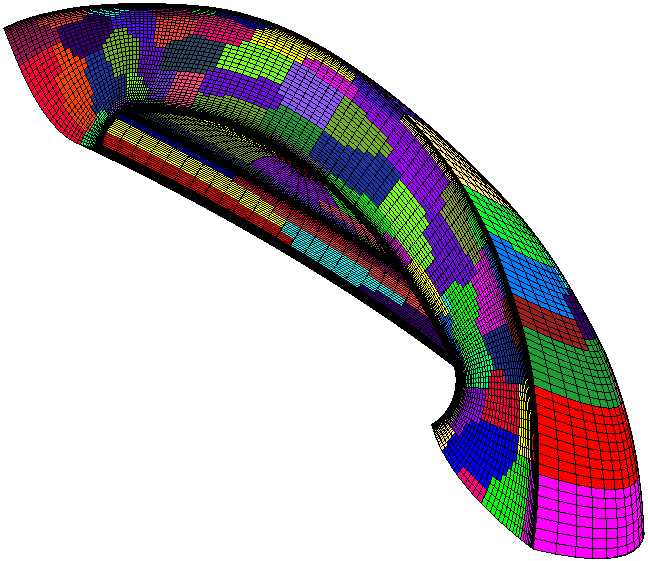
\includegraphics[width=.45\textwidth]{capsule_partitioned}

        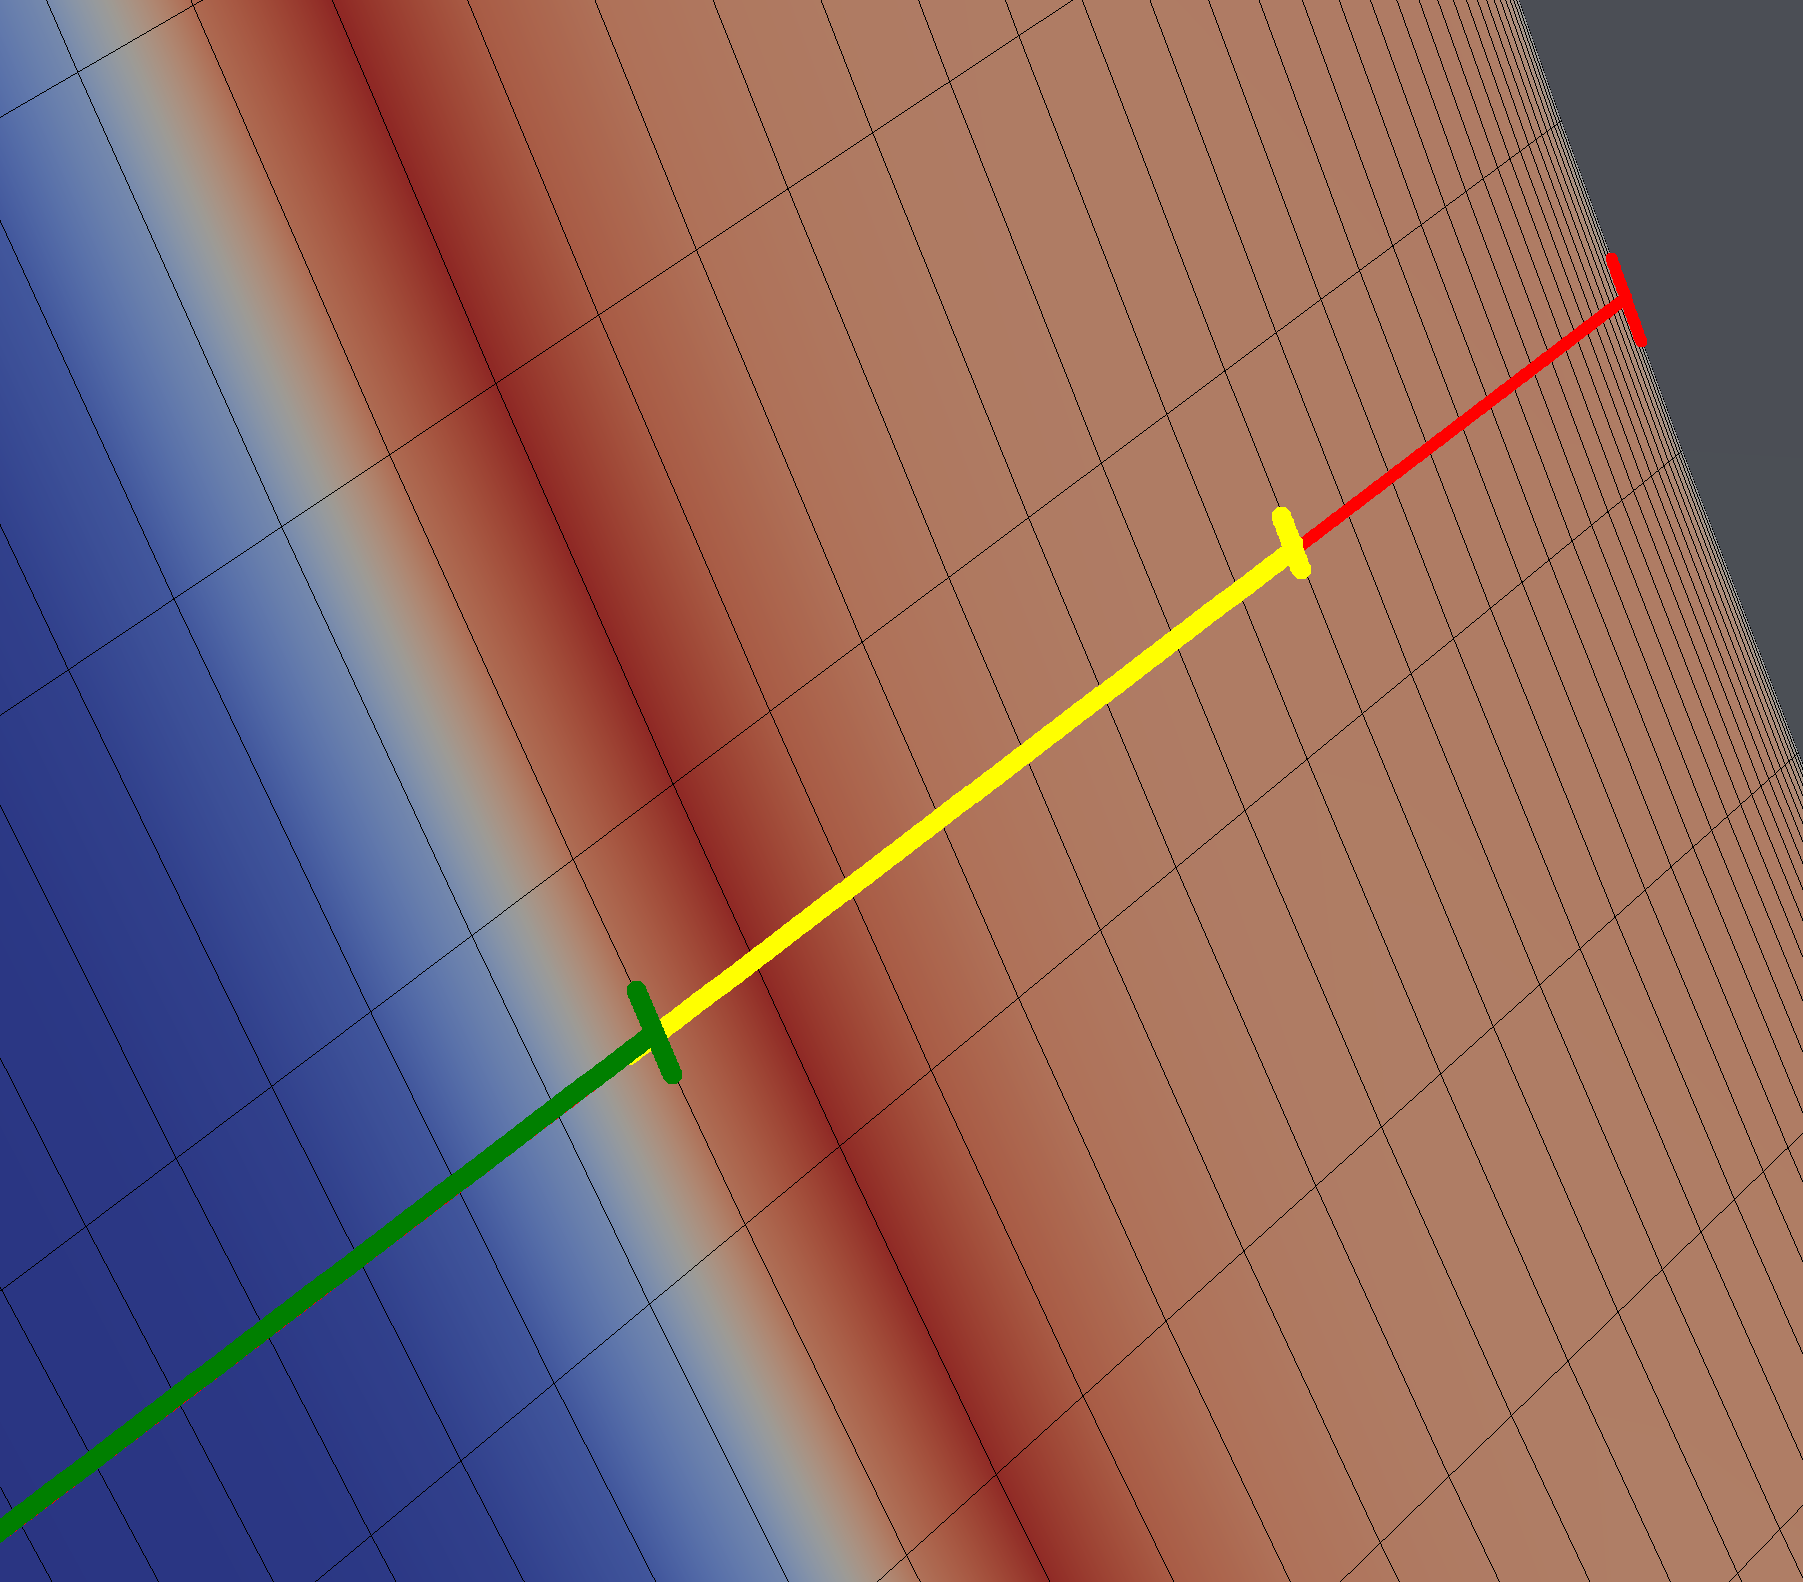
\includegraphics[width=.45\textwidth]{fins-transition} \;
        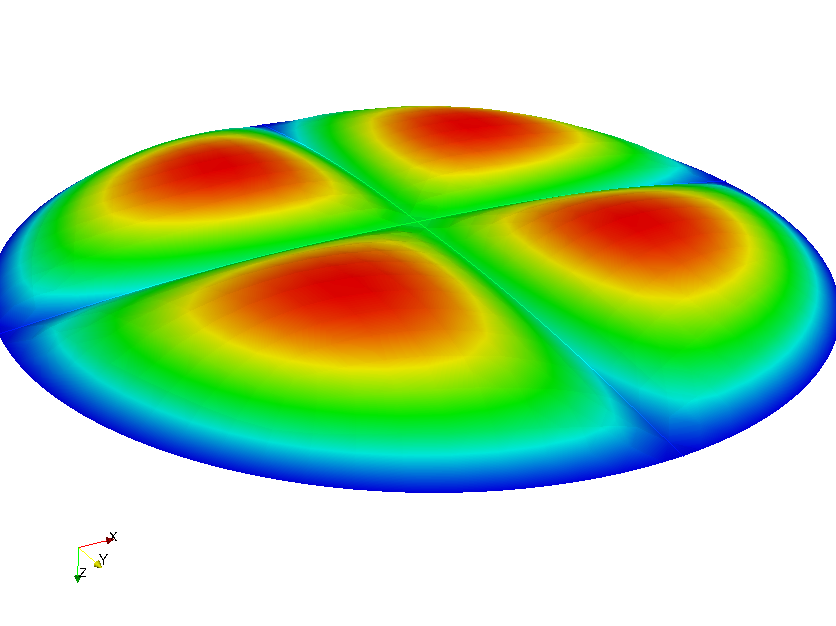
\includegraphics[width=.45\textwidth]{sheet_perspective}

      \end{center}
  \end{columns}
\end{frame}

